\chapter{Clusterização como pré-processamento na compressão de textos}
Nos capítulos anteriores, construímos a estrutura teórica necessária para compreender a \emph{compressão de texto} e sua relação com a \emph{teoria da informação}.
Fica claro que os algoritmos apresentados, tomam vantagem de alguma redundância presente na mensagem para representar a informação de maneira mais eficiente.
Isto é, a \textbf{eficiência} destes algoritmos está intimamente ligada com a \textbf{entropia} do texto a ser comprimido,
 nos dando um indício de que \textbf{minimizar} a entropia, pode ser uma forma de \textbf{maximizar} a \textbf{taxa de compressão}.
 
O capítulo~\ref{cap:clus} apresenta uma técnica para organizar o texto em \emph{grupos de mensagens similares} (\textbf{clusterização}), o que significa diminuir a variação de termos dentro de cada cluster (ou reduzir a sua \textbf{entropia}).
Neste capítulo, exploraremos de maneira empírica a relação entre a entropia associada a um texto e a taxa de compressão dos algoritmos apresentados no capítulo~\ref{cap:comp}.

A seguir, será descrito um experimento que utiliza a \textbf{clusterização} como pré-processamento de uma base de dados textual, visando uma melhora na performance dos algoritmos de compressão \emph{sem perda}.
Foram realizados experimentos utilizando ou não o pré-processamento, afim de medir o impacto da clusterização para os algoritmos testados (que serão listados em seções posteriores).

Todo o projeto foi desenvolvido em \emph{Python} (principalmente ao seu vasto ferramental para manipulação de dados) e o código está disponível no GitHub [TODO REF GITHUB].
O código fonte está organizado nas seguintes camadas:
\begin{itemize}
	\item \textbf{dataset}: Contém os arquivos \emph{.csv} que serão carregados como base de dados.
	\item \textbf{compressors}: Classes e scripts com a implementação dos codificadores utilizados.
	\item \textbf{stackexchange\_compression\_experiments.ipynb}: \emph{Python notebook} com o código fonte de todo o experimento (pré-processamento dos dados, particionamento das bases, aplicação dos algoritmos de compressão, plot de gráficos, entre outros).
\end{itemize}
\pagebreak

\section{Escolha e tratamento de dados}
Para a realização do experimento, a escolha da base de dados é uma etapa primordial.
É necessária uma base de dados robusta, com uma grande quantidade de \textbf{texto} e que permita a criação de \emph{clusters} contendo assuntos diversos.

Para o experimento, foram selecionados os dados do desafio ``\emph{Transfer Learning o Stack Exchange Tags}''  disponível no \emph{kaggle}.
Trata-se de um conjunto de dados extraídos do website \emph{Stack Exchange}, basicamente um \textbf{fórum online} sobre os mais variados assuntos (ou seja, alta quantidade de textos de diferentes naturezas).

O \emph{dataset} tem como principais informações o título das questões, o conteúdo da questões (em formato HTML) e as \emph{tags} que classificam o conteúdo em diversos tópicos (biologia, culinária, criptografia, robótica e viagem).
O \emph{dataset} original possui um tamanho aproximado de \textbf{50MB}. 

\subsection{Criação do dataframe principal}
Os dados extraídos do \emph{kaggle} estão originalmente em arquivos \emph{csv}, um arquivo para cada tópico.
Portanto, para executar o experimento de compressão, precisamos unir os arquivos em um único \emph{dataframe}.
Para cada arquivo, selecionamos \textbf{1500} linhas (devido as limitações do hardware utilizado para o teste), o \emph{dataframe} final gerado possuí aproximadamente \textbf{7MB} de informação.


\begin{lstlisting}[language=Python, caption=Carregando base de dados]
# Loading dataframe
def load_dataset(dataset_name):
    f_path = 'dataset/stack-exchange-tags/{dataset}.csv'.format(dataset = dataset_name)
    full_path = os.path.join(os.getcwd(), f_path)
    return p.read_csv(full_path, index_col=0, nrows=1500)

ds_names = ['biology', 'cooking', 'crypto', 'diy', 'robotics', 'travel']
frames = [load_dataset(name) for name in ds_names]
df = p.concat(frames)
\end{lstlisting}

\subsection{Sanitização das colunas}
Como parte da preparação dos dados para o experimento, realizamos a sanitização das colunas do \emph{dataframe}.
Nessa etapa, removemos as \emph{stopwords}, pontuações, tags \emph{html} e outras informações que podem ser problemáticas para o processo de clusterização.
Vale salientar que, a sanitização é aplicada apenas como pré-processamento para a clusterização (basicamente, utilizaremos a informação para particionar os dados antes de comprimi-los).

\begin{lstlisting}[language=Python, caption=Sanitização do texto]
from wordcloud import STOPWORDS
import re\
stop_words = set(STOPWORDS)

# # Sanitizing columns
def sanitize_column(data):
    # convert to lower
    data = data.lower()
    # strip html
    data = re.sub(r'\<[^<>]*\>','',data.lower())
    #removing pontuation
    data = re.sub(r'[^a-zA-Z0-9]',' ',data)
    # Remove new lines and tabs
    data = re.sub(r'\s',' ',data)

    #strip data
    data = data.strip()

    #Spling words
    data = data.split()
    
    #Remove extra blank space
    data = list(filter(lambda s: s != ' ', data))

    # Remove stop words
    data =  list(filter(lambda s: s not in stop_words,data))

    #remove single chars words
    data = list(filter(lambda s: len(s) > 1, data))

    return data
def array_column_to_text(column):
    text = ''
    for w in column:
        for s in w:
            text += ' ' + s 
    return text
df['sanitezed_content'] = df['content'].apply(sanitize_column)
\end{lstlisting}

A biblioteca \textbf{worldcloud} nos permite visualizar a frequência de cada palavras de maneira gráfica.
A imagem a seguir mostra a representação dos conteúdo após a sanitização, dando destaque para as palavras mais frequentes.

 \begin{figure}[H]
   \centering
   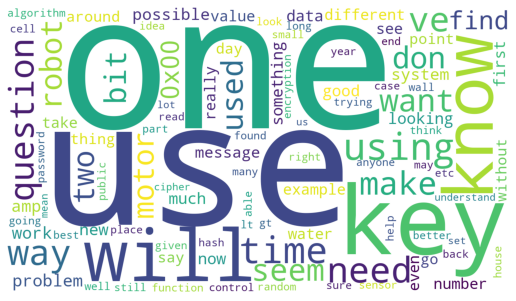
\includegraphics[scale=0.50]{figs/wordcloud1.png}
    \caption{Cluster de palavras}
    \label{fig:wordcloud1}
 \end{figure}

\section{Compressão de textos}
Os experimentos foram realizados com dois algoritmos clássicos de compressão \emph{sem perda} e suas versões baseadas em palavras (\textbf{Huffman}, \textbf{Huffword}, \textbf{LZ77}, \textbf{WLZ77}).
Com estes algoritmos, teremos uma comparação do efeito da clusterização entre um algoritmo baseado em \textbf{probabilidades} (Huffman)  e outro baseado em \textbf{dicionário} (LZ77).
Espera-se que com a versão baseado em palavras, o impacto da clusterização na taxa de compressão seja ainda maior (já que os clusters são formados a nível de palavras).
A seguir, serão descritos alguns detalhes específicos da implementação dos compressores para o experimento (principalmente os detalhes não contidos no algoritmo formal apresentado no Capítulo~\ref{cap:comp}).

\subsection{Classes auxiliares}
Para facilitar a reutilização de código na aplicação dos diferentes compressores, criamos a classe auxiliar (\emph{TextCompressor}).
Nesta classe são expostos os método \emph{encode(text)} e \emph{decode()}, que servem como um ``contrato'' para a implementação dos algoritmos de compressão.

\begin{lstlisting}[language=Python, caption=Classe TextCompressor]
class TextCompressor:
    def __init__(self):
        self.originaltext = None
        self.stats = None
    def encode(self, text):
        self.originaltext = text
        pass
    def decode(self):
        pass
\end{lstlisting}

Cada \emph{classe} específica de compressor herda da classe base \emph{TextCompressor}, criando sua própria implementação dos métodos \emph{encode} e \emph{decode}.

Outra classe auxiliar implementada foi a \emph{CompressionStats}. Trata-se de uma interface para padronizar a leitura das métricas sobre os compressores.
\begin{lstlisting}[language=Python, caption=Implementaçào da classe base CompressionStats]
class CompressionStats:
    def _avg_code(self):
        return (self.compressedtextsize / self.originaltextsize) * 8
    def _compression_rate(self):
        return 100 - (self.compressedtextsize / self.originaltextsize) * 100
    def __init__(self, originaltext, compressedtext):
        self.originaltextsize = len(originaltext)
        self.compressedtextsize = len(compressedtext)
    def __str__(self) -> str:
        return stats_text.format(csize=self._avg_code(), osize=self.originaltextsize, nsize=self.compressedtextsize, crate=self._compression_rate())
\end{lstlisting}

\subsection{Compressão baseada em palavras}
Para a implementação dos algoritmos baseados em \textbf{palavras}, boa parte do código fonte utilizado nos algoritmos ``canônicos'' foram reutilizados.
Como o \emph{Python} é uma linguagem de \textbf{tipagem dinâmica}, a implementação ``canônica'' interpreta a entrada como um vetor de \emph{símbolos} (sem necessariamente distinguir o tipo de símbolo).
Isso permite uma maior flexibilidade para o reaproveitamento de grande parte das funções escritas, independente do alfabeto de origem utilizado. 

Conforme descrito no Capítulo~\ref{cap:comp}, o \emph{Huffword} computa as \emph{palavras} e \emph{separadores} como duas entradas distintas.
Para dividir a entrada entre \emph{palavras} e \emph{separadores}, utilizamos a biblioteca \emph{re}, que permite executar buscas em \emph{strings} utilizando \emph{regex}.
Basicamente, executamos uma busca na entrada pelas \emph{palavras} e atribuímos à variável \emph{words} (o mesmo vale para os separadores, que foram atribuídos a variável \emph{non\_words}).

\begin{lstlisting}[language=Python, caption=Função \emph{encode} para o \emph{Huffword}]
def _build_huffword_code(seq):
    freqs = frequency_dictionary(seq)
    huff_tree = canonical.build_huff_tree(freqs)
    code_table= canonical.build_code_table(huff_tree)
    return code_table
    
def huffword_encode(text):
    # Words huff tree
    words = re.findall(r'\w+', text)
    words_code = _build_huffword_code(words)

    # Non words huff tree
    nonwords = re.findall(r'\W+', text)
    nonwords_code = _build_huffword_code(nonwords)

    encoded_string = ""

    # When text start with non-word append 0, otherwise append 1
    starts_with = 0
    if text.startswith(words[0]):
        starts_with += 1
    
    # Append starts with as the first char
    encoded_string += str(starts_with)

    # Encode intercalating words and nonwords
    w_index = 0
    nw_index = 0

    #When starts with non words
    if not starts_with:
        encoded_string += nonwords_code[nonwords[0]]
    
    while w_index < len(words) or nw_index < len(nonwords):
        if w_index < len(words):
            word = words[w_index]
            encoded_string += words_code[word]
            w_index += 1
        
        if nw_index < len(nonwords):
            nonword = nonwords[nw_index]
            encoded_string += nonwords_code[nonword]
            nw_index += 1
    
    return {'encoded' : encoded_string,
            'words_meta' : (words, words_code),
            'non_words_meta': (nonwords, nonwords_code)}
\end{lstlisting}



\section{Partição de dados}
Para o propósito do experimento, a base de dados foi comprimida a partir de dois métodos diferentes de partição.
Na primeira, os dados são particionados \textbf{aleatoriamente} em $n$ partes.
Já para o teste da clusterização, agrupamos os mesmos dados em $n$ \emph{clusters} criados pelo algoritmo \emph{k-means}.
Cada algoritmo de compressão é executado sobre as $n$ partições (grupos), e as métricas são computadas como uma média aritmética do desempenho alcançado em cada partição.

\subsection{Partição aleatória}
A partição aleatória consiste em dividir o \emph{dataframe} original em $n$ novos \emph{dataframes}.
Para evitar possíveis \emph{bias} presentes na base original (por exemplo, se os dados já estivessem originalmente agrupados), precisamos que essa divisão seja aleatória. 

Para isso, foi utilizado o método $.sample()$, que retorna uma amostra aleatória de items. 
O parâmetro $frac=1$, faz com que o método retorne uma amostra com todos os dados (porém de maneira randômica).
Depois disso, fracionamos o array utilizando a função $array\_split()$ da biblioteca $numpy$.

\begin{lstlisting}[language=Python, caption=Partição aleatória de dados]
# Data to compress: Compress the original data raw
raw_text = df['content']

#Shuffle raw text
shuffle = raw_text.sample(frac=1)
partitions = np.array_split(shuffle, n_partitions)
\end{lstlisting}

\subsection{Clusterizacao}
Tecnologia e implementação
Mostrar parametros
mostrar gráficos

\section{Resultados}
\subsection{Metodologia}
Explicar sobre a extassao de medidas de comparacao

\subsection{Resultados pré clusterizacao}

\subsection{Resultados pós clusterizacao}

\section{Conclusao}

\section{Trabalhos relacionados e melhorias}




